% Options for packages loaded elsewhere
\PassOptionsToPackage{unicode}{hyperref}
\PassOptionsToPackage{hyphens}{url}
%
\documentclass[
]{article}
\usepackage{amsmath,amssymb}
\usepackage{iftex}
\ifPDFTeX
  \usepackage[T1]{fontenc}
  \usepackage[utf8]{inputenc}
  \usepackage{textcomp} % provide euro and other symbols
\else % if luatex or xetex
  \usepackage{unicode-math} % this also loads fontspec
  \defaultfontfeatures{Scale=MatchLowercase}
  \defaultfontfeatures[\rmfamily]{Ligatures=TeX,Scale=1}
\fi
\usepackage{lmodern}
\ifPDFTeX\else
  % xetex/luatex font selection
\fi
% Use upquote if available, for straight quotes in verbatim environments
\IfFileExists{upquote.sty}{\usepackage{upquote}}{}
\IfFileExists{microtype.sty}{% use microtype if available
  \usepackage[]{microtype}
  \UseMicrotypeSet[protrusion]{basicmath} % disable protrusion for tt fonts
}{}
\makeatletter
\@ifundefined{KOMAClassName}{% if non-KOMA class
  \IfFileExists{parskip.sty}{%
    \usepackage{parskip}
  }{% else
    \setlength{\parindent}{0pt}
    \setlength{\parskip}{6pt plus 2pt minus 1pt}}
}{% if KOMA class
  \KOMAoptions{parskip=half}}
\makeatother
\usepackage{xcolor}
\usepackage[margin=1in]{geometry}
\usepackage{color}
\usepackage{fancyvrb}
\newcommand{\VerbBar}{|}
\newcommand{\VERB}{\Verb[commandchars=\\\{\}]}
\DefineVerbatimEnvironment{Highlighting}{Verbatim}{commandchars=\\\{\}}
% Add ',fontsize=\small' for more characters per line
\usepackage{framed}
\definecolor{shadecolor}{RGB}{248,248,248}
\newenvironment{Shaded}{\begin{snugshade}}{\end{snugshade}}
\newcommand{\AlertTok}[1]{\textcolor[rgb]{0.94,0.16,0.16}{#1}}
\newcommand{\AnnotationTok}[1]{\textcolor[rgb]{0.56,0.35,0.01}{\textbf{\textit{#1}}}}
\newcommand{\AttributeTok}[1]{\textcolor[rgb]{0.13,0.29,0.53}{#1}}
\newcommand{\BaseNTok}[1]{\textcolor[rgb]{0.00,0.00,0.81}{#1}}
\newcommand{\BuiltInTok}[1]{#1}
\newcommand{\CharTok}[1]{\textcolor[rgb]{0.31,0.60,0.02}{#1}}
\newcommand{\CommentTok}[1]{\textcolor[rgb]{0.56,0.35,0.01}{\textit{#1}}}
\newcommand{\CommentVarTok}[1]{\textcolor[rgb]{0.56,0.35,0.01}{\textbf{\textit{#1}}}}
\newcommand{\ConstantTok}[1]{\textcolor[rgb]{0.56,0.35,0.01}{#1}}
\newcommand{\ControlFlowTok}[1]{\textcolor[rgb]{0.13,0.29,0.53}{\textbf{#1}}}
\newcommand{\DataTypeTok}[1]{\textcolor[rgb]{0.13,0.29,0.53}{#1}}
\newcommand{\DecValTok}[1]{\textcolor[rgb]{0.00,0.00,0.81}{#1}}
\newcommand{\DocumentationTok}[1]{\textcolor[rgb]{0.56,0.35,0.01}{\textbf{\textit{#1}}}}
\newcommand{\ErrorTok}[1]{\textcolor[rgb]{0.64,0.00,0.00}{\textbf{#1}}}
\newcommand{\ExtensionTok}[1]{#1}
\newcommand{\FloatTok}[1]{\textcolor[rgb]{0.00,0.00,0.81}{#1}}
\newcommand{\FunctionTok}[1]{\textcolor[rgb]{0.13,0.29,0.53}{\textbf{#1}}}
\newcommand{\ImportTok}[1]{#1}
\newcommand{\InformationTok}[1]{\textcolor[rgb]{0.56,0.35,0.01}{\textbf{\textit{#1}}}}
\newcommand{\KeywordTok}[1]{\textcolor[rgb]{0.13,0.29,0.53}{\textbf{#1}}}
\newcommand{\NormalTok}[1]{#1}
\newcommand{\OperatorTok}[1]{\textcolor[rgb]{0.81,0.36,0.00}{\textbf{#1}}}
\newcommand{\OtherTok}[1]{\textcolor[rgb]{0.56,0.35,0.01}{#1}}
\newcommand{\PreprocessorTok}[1]{\textcolor[rgb]{0.56,0.35,0.01}{\textit{#1}}}
\newcommand{\RegionMarkerTok}[1]{#1}
\newcommand{\SpecialCharTok}[1]{\textcolor[rgb]{0.81,0.36,0.00}{\textbf{#1}}}
\newcommand{\SpecialStringTok}[1]{\textcolor[rgb]{0.31,0.60,0.02}{#1}}
\newcommand{\StringTok}[1]{\textcolor[rgb]{0.31,0.60,0.02}{#1}}
\newcommand{\VariableTok}[1]{\textcolor[rgb]{0.00,0.00,0.00}{#1}}
\newcommand{\VerbatimStringTok}[1]{\textcolor[rgb]{0.31,0.60,0.02}{#1}}
\newcommand{\WarningTok}[1]{\textcolor[rgb]{0.56,0.35,0.01}{\textbf{\textit{#1}}}}
\usepackage{graphicx}
\makeatletter
\def\maxwidth{\ifdim\Gin@nat@width>\linewidth\linewidth\else\Gin@nat@width\fi}
\def\maxheight{\ifdim\Gin@nat@height>\textheight\textheight\else\Gin@nat@height\fi}
\makeatother
% Scale images if necessary, so that they will not overflow the page
% margins by default, and it is still possible to overwrite the defaults
% using explicit options in \includegraphics[width, height, ...]{}
\setkeys{Gin}{width=\maxwidth,height=\maxheight,keepaspectratio}
% Set default figure placement to htbp
\makeatletter
\def\fps@figure{htbp}
\makeatother
\setlength{\emergencystretch}{3em} % prevent overfull lines
\providecommand{\tightlist}{%
  \setlength{\itemsep}{0pt}\setlength{\parskip}{0pt}}
\setcounter{secnumdepth}{-\maxdimen} % remove section numbering
\ifLuaTeX
  \usepackage{selnolig}  % disable illegal ligatures
\fi
\IfFileExists{bookmark.sty}{\usepackage{bookmark}}{\usepackage{hyperref}}
\IfFileExists{xurl.sty}{\usepackage{xurl}}{} % add URL line breaks if available
\urlstyle{same}
\hypersetup{
  pdftitle={Regresión Logística Ordinal},
  hidelinks,
  pdfcreator={LaTeX via pandoc}}

\title{Regresión Logística Ordinal}
\author{}
\date{\vspace{-2.5em}}

\begin{document}
\maketitle

{
\setcounter{tocdepth}{2}
\tableofcontents
}
\begin{flushleft}
\includegraphics[width=0.3\linewidth]{logoPUCP} \end{flushleft}

\hypertarget{facultad-de-ciencias-sociales---pucp}{%
\subsection{\texorpdfstring{\textbf{FACULTAD DE CIENCIAS SOCIALES -
PUCP}
}{FACULTAD DE CIENCIAS SOCIALES - PUCP  }}\label{facultad-de-ciencias-sociales---pucp}}

\hypertarget{curso-pol-304---estaduxedstica-para-el-anuxe1lisis-poluxedtico-2-semestre-2024---2}{%
\subsubsection{Curso: POL 304 - Estadística para el análisis político 2
\textbar{} Semestre 2024 -
2}\label{curso-pol-304---estaduxedstica-para-el-anuxe1lisis-poluxedtico-2-semestre-2024---2}}

\hypertarget{jefas-de-pruxe1ctica-karina-alcuxe1ntara-y-lizette-crispuxedn}{%
\paragraph{\texorpdfstring{Jefas de Práctica: Karina Alcántara 👩‍🏫 y
Lizette Crispín
👩‍🏫}{Jefas de Práctica: Karina Alcántara 👩‍🏫 y Lizette Crispín 👩‍🏫 }}\label{jefas-de-pruxe1ctica-karina-alcuxe1ntara-y-lizette-crispuxedn}}

Llamemos a los paquetes

\begin{Shaded}
\begin{Highlighting}[]
\FunctionTok{library}\NormalTok{(rio) }\CommentTok{\#para importar la base}
\FunctionTok{library}\NormalTok{(fastDummies) }\CommentTok{\#Para volver dummy a una variable categórica}
\FunctionTok{library}\NormalTok{(MASS) }\CommentTok{\#para crear el modelo}
\FunctionTok{library}\NormalTok{(marginaleffects) }\CommentTok{\#para calcular la probabilidad}
\FunctionTok{library}\NormalTok{(DescTools) }\CommentTok{\#Para calcular el pseudo R2}
\FunctionTok{library}\NormalTok{(dplyr)}
\end{Highlighting}
\end{Shaded}

\begin{Shaded}
\begin{Highlighting}[]
\NormalTok{data }\OtherTok{\textless{}{-}} \FunctionTok{import}\NormalTok{(}\StringTok{"trabajadores.sav"}\NormalTok{)}
\end{Highlighting}
\end{Shaded}

\begin{Shaded}
\begin{Highlighting}[]
\FunctionTok{names}\NormalTok{(data)}
\end{Highlighting}
\end{Shaded}

\begin{verbatim}
##  [1] "id"              "sexo"            "fechnac"         "educ"           
##  [5] "catlab"          "salario_actual"  "salario_inicial" "antiguedad"     
##  [9] "experiencia"     "minoría"         "directivo"
\end{verbatim}

\textbf{Pregunta de investigación:}

\hypertarget{quuxe9-factores-condicionan-el-nivel-de-salario-que-puede-tener-un-trabajador}{%
\subsection{\texorpdfstring{\textbf{¿Qué factores condicionan el nivel
de salario que puede tener un
trabajador@?}}{¿Qué factores condicionan el nivel de salario que puede tener un trabajador@?}}\label{quuxe9-factores-condicionan-el-nivel-de-salario-que-puede-tener-un-trabajador}}

\hypertarget{modelo-1-de-quuxe9-manera-el-sexo-y-los-auxf1os-de-educaciuxf3n-condicionan-el-nivel-de-salario-que-puede-tener-un-trabajador}{%
\section{\texorpdfstring{Modelo 1: \textbf{¿De qué manera, el sexo y los
años de educación condicionan el nivel de salario que puede tener un
trabajador?}}{Modelo 1: ¿De qué manera, el sexo y los años de educación condicionan el nivel de salario que puede tener un trabajador?}}\label{modelo-1-de-quuxe9-manera-el-sexo-y-los-auxf1os-de-educaciuxf3n-condicionan-el-nivel-de-salario-que-puede-tener-un-trabajador}}

\hypertarget{paso-1-preparar-la-data}{%
\subsection{\texorpdfstring{\textbf{Paso 1: Preparar la
data}}{Paso 1: Preparar la data}}\label{paso-1-preparar-la-data}}

\hypertarget{variable-dependiente-salario-anual-nivel}{%
\subsubsection{Variable dependiente: Salario anual
(nivel)}\label{variable-dependiente-salario-anual-nivel}}

Está como un número, identificamos los cuartiles para poder realizar 3
cortes y crear cuatro categorías.

\begin{Shaded}
\begin{Highlighting}[]
\FunctionTok{summary}\NormalTok{(data}\SpecialCharTok{$}\NormalTok{salario\_actual)}
\end{Highlighting}
\end{Shaded}

\begin{verbatim}
##    Min. 1st Qu.  Median    Mean 3rd Qu.    Max. 
##   15750   24000   28875   34420   36938  135000
\end{verbatim}

\begin{Shaded}
\begin{Highlighting}[]
\FunctionTok{hist}\NormalTok{(data}\SpecialCharTok{$}\NormalTok{salario\_actual)}
\end{Highlighting}
\end{Shaded}

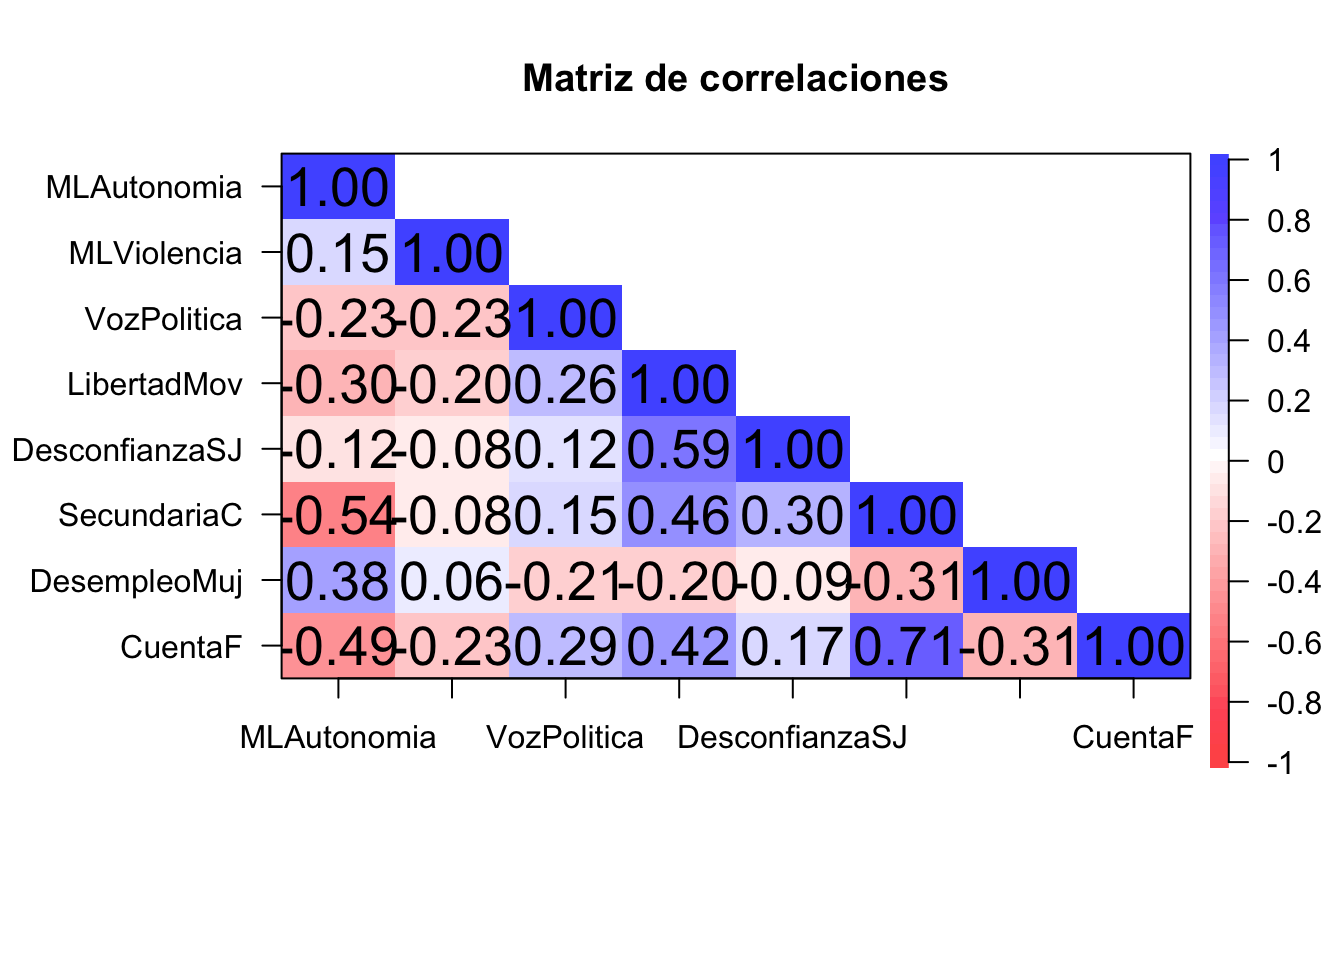
\includegraphics{pd5_files/figure-latex/unnamed-chunk-5-1.pdf}

Inidcamos los puntos de corte, guiándonos de los cuartiles, el resultado
nos dará un factor ordenado.

\begin{Shaded}
\begin{Highlighting}[]
\NormalTok{data}\SpecialCharTok{$}\NormalTok{salario\_actual\_ordinal }\OtherTok{\textless{}{-}} \FunctionTok{cut}\NormalTok{(data}\SpecialCharTok{$}\NormalTok{salario\_actual, }\AttributeTok{breaks =} \FunctionTok{c}\NormalTok{(}\DecValTok{0}\NormalTok{, }\DecValTok{24000}\NormalTok{,}\DecValTok{28875}\NormalTok{, }\DecValTok{36938}\NormalTok{,}\DecValTok{135000}\NormalTok{),}
                                  \AttributeTok{include.lowest =}\NormalTok{ T, }\AttributeTok{ordered\_result =}\NormalTok{ T,}
                                  \AttributeTok{labels =} \FunctionTok{c}\NormalTok{(}\StringTok{"Muy Bajo"}\NormalTok{, }\StringTok{"Bajo"}\NormalTok{,}
                                        \StringTok{"Alto"}\NormalTok{, }\StringTok{"Muy Alto"}\NormalTok{))}

\FunctionTok{table}\NormalTok{(data}\SpecialCharTok{$}\NormalTok{salario\_actual\_ordinal)}
\end{Highlighting}
\end{Shaded}

\begin{verbatim}
## 
## Muy Bajo     Bajo     Alto Muy Alto 
##      120      117      118      119
\end{verbatim}

\hypertarget{variables-independientes-sexo-y-educaciuxf3n}{%
\subsubsection{Variables independientes: sexo y
educación}\label{variables-independientes-sexo-y-educaciuxf3n}}

\begin{itemize}
\tightlist
\item
  Sexo: identifiquemos como está y de ser necesario recategoricemos y
  agreguemos etiquetas.
\end{itemize}

\begin{Shaded}
\begin{Highlighting}[]
\FunctionTok{class}\NormalTok{(data}\SpecialCharTok{$}\NormalTok{sexo)}
\end{Highlighting}
\end{Shaded}

\begin{verbatim}
## [1] "numeric"
\end{verbatim}

\begin{Shaded}
\begin{Highlighting}[]
\FunctionTok{table}\NormalTok{(data}\SpecialCharTok{$}\NormalTok{sexo)}
\end{Highlighting}
\end{Shaded}

\begin{verbatim}
## 
##   0   1 
## 216 258
\end{verbatim}

\begin{Shaded}
\begin{Highlighting}[]
\NormalTok{data }\OtherTok{\textless{}{-}}\NormalTok{ data }\SpecialCharTok{\%\textgreater{}\%} 
  \FunctionTok{mutate}\NormalTok{(}\AttributeTok{sexo =} \FunctionTok{factor}\NormalTok{(sexo, }\AttributeTok{levels =} \DecValTok{0}\SpecialCharTok{:}\DecValTok{1}\NormalTok{, }\AttributeTok{labels =} \FunctionTok{c}\NormalTok{(}\StringTok{"Mujer"}\NormalTok{, }\StringTok{"Hombre"}\NormalTok{)))}
\FunctionTok{table}\NormalTok{(data}\SpecialCharTok{$}\NormalTok{sexo)}
\end{Highlighting}
\end{Shaded}

\begin{verbatim}
## 
##  Mujer Hombre 
##    216    258
\end{verbatim}

Convertimos a dummy a la variable sexo

\begin{Shaded}
\begin{Highlighting}[]
\NormalTok{data}\OtherTok{\textless{}{-}}\FunctionTok{dummy\_cols}\NormalTok{(data, }\AttributeTok{select\_columns =} \FunctionTok{c}\NormalTok{(}\StringTok{"sexo"}\NormalTok{))}
\end{Highlighting}
\end{Shaded}

\begin{itemize}
\tightlist
\item
  Educación: Identifiquemos como está
\end{itemize}

\begin{Shaded}
\begin{Highlighting}[]
\FunctionTok{str}\NormalTok{(data}\SpecialCharTok{$}\NormalTok{educ)}
\end{Highlighting}
\end{Shaded}

\begin{verbatim}
##  num [1:474] 15 16 12 8 15 15 15 12 15 12 ...
##  - attr(*, "label")= chr "Nivel educativo"
##  - attr(*, "format.spss")= chr "F2.0"
##  - attr(*, "display_width")= int 9
##  - attr(*, "labels")= Named num [1:11] 0 8 12 14 15 16 17 18 19 20 ...
##   ..- attr(*, "names")= chr [1:11] "0 (Ausente)" "8" "12" "14" ...
\end{verbatim}

Revisamos que se hayan añadido nuestras variables correctamente.

\begin{Shaded}
\begin{Highlighting}[]
\FunctionTok{names}\NormalTok{(data)}
\end{Highlighting}
\end{Shaded}

\begin{verbatim}
##  [1] "id"                     "sexo"                   "fechnac"               
##  [4] "educ"                   "catlab"                 "salario_actual"        
##  [7] "salario_inicial"        "antiguedad"             "experiencia"           
## [10] "minoría"                "directivo"              "salario_actual_ordinal"
## [13] "sexo_Mujer"             "sexo_Hombre"
\end{verbatim}

Veamos si el nivel educativo, y el ser mujer influye en el salario
actual

\hypertarget{paso-2-creaciuxf3n-del-modelo}{%
\subsection{\texorpdfstring{\textbf{Paso 2: Creación del
modelo}}{Paso 2: Creación del modelo}}\label{paso-2-creaciuxf3n-del-modelo}}

\begin{Shaded}
\begin{Highlighting}[]
\NormalTok{modelo }\OtherTok{\textless{}{-}} \FunctionTok{polr}\NormalTok{(salario\_actual\_ordinal }\SpecialCharTok{\textasciitilde{}}\NormalTok{ sexo\_Mujer }\SpecialCharTok{+}\NormalTok{ educ, }\AttributeTok{data =}\NormalTok{ data, }\AttributeTok{Hess =}\NormalTok{ T)}
\FunctionTok{summary}\NormalTok{(modelo)}
\end{Highlighting}
\end{Shaded}

\begin{verbatim}
## Call:
## polr(formula = salario_actual_ordinal ~ sexo_Mujer + educ, data = data, 
##     Hess = T)
## 
## Coefficients:
##              Value Std. Error t value
## sexo_Mujer -1.8363    0.20268   -9.06
## educ        0.4618    0.04136   11.17
## 
## Intercepts:
##               Value   Std. Error t value
## Muy Bajo|Bajo  3.6632  0.5566     6.5811
## Bajo|Alto      5.3306  0.5752     9.2669
## Alto|Muy Alto  7.1165  0.6214    11.4515
## 
## Residual Deviance: 1000.749 
## AIC: 1010.749
\end{verbatim}

\hypertarget{veamos-el-p-value-y-determinar-la-significancia-de-las-variables-independientes}{%
\subsubsection{Veamos el p-value y determinar la significancia de las
variables
independientes}\label{veamos-el-p-value-y-determinar-la-significancia-de-las-variables-independientes}}

Guardamos la tabla de coeficientes en un objeto.

\begin{Shaded}
\begin{Highlighting}[]
\NormalTok{summary\_table }\OtherTok{\textless{}{-}} \FunctionTok{coef}\NormalTok{(}\FunctionTok{summary}\NormalTok{(modelo)) }\CommentTok{\#OBTENER TABLA CON COEFICIENTES}
\NormalTok{summary\_table}
\end{Highlighting}
\end{Shaded}

\begin{verbatim}
##                    Value Std. Error   t value
## sexo_Mujer    -1.8362608 0.20267681 -9.060044
## educ           0.4618446 0.04136102 11.166180
## Muy Bajo|Bajo  3.6632440 0.55662857  6.581128
## Bajo|Alto      5.3305723 0.57522584  9.266921
## Alto|Muy Alto  7.1165070 0.62144567 11.451535
\end{verbatim}

Calculamos el p-value a partir de t-value y lo almacenamos en otro
objeto.

\begin{Shaded}
\begin{Highlighting}[]
\NormalTok{pval }\OtherTok{\textless{}{-}} \FunctionTok{pnorm}\NormalTok{(}\FunctionTok{abs}\NormalTok{(summary\_table[, }\StringTok{"t value"}\NormalTok{]),}\AttributeTok{lower.tail =} \ConstantTok{FALSE}\NormalTok{)}\SpecialCharTok{*} \DecValTok{2}
\NormalTok{pval}
\end{Highlighting}
\end{Shaded}

\begin{verbatim}
##    sexo_Mujer          educ Muy Bajo|Bajo     Bajo|Alto Alto|Muy Alto 
##  1.303979e-19  5.969318e-29  4.668919e-11  1.915972e-20  2.310177e-30
\end{verbatim}

Agregamos este nuevo objeto (vector) a la tabla de coeficientes.

\begin{Shaded}
\begin{Highlighting}[]
\NormalTok{summary\_table }\OtherTok{\textless{}{-}} \FunctionTok{cbind}\NormalTok{(summary\_table, }\StringTok{"p value"} \OtherTok{=}\NormalTok{ pval)}
\NormalTok{summary\_table}
\end{Highlighting}
\end{Shaded}

\begin{verbatim}
##                    Value Std. Error   t value      p value
## sexo_Mujer    -1.8362608 0.20267681 -9.060044 1.303979e-19
## educ           0.4618446 0.04136102 11.166180 5.969318e-29
## Muy Bajo|Bajo  3.6632440 0.55662857  6.581128 4.668919e-11
## Bajo|Alto      5.3305723 0.57522584  9.266921 1.915972e-20
## Alto|Muy Alto  7.1165070 0.62144567 11.451535 2.310177e-30
\end{verbatim}

Esta tabla nos da un resumen de los coeficientes y el pvalue.

\begin{itemize}
\tightlist
\item
  H0: La variable independiente no aporta al modelo
\end{itemize}

Lo que buscamos entonces es ver \emph{si el p-value es menor a 0.05} en
las variables independientes seleccionadas.

\hypertarget{paso-3-interpretamos-el-efecto-de-las-variables}{%
\subsection{\texorpdfstring{\textbf{Paso 3: Interpretamos el efecto de
las
variables}}{Paso 3: Interpretamos el efecto de las variables}}\label{paso-3-interpretamos-el-efecto-de-las-variables}}

\begin{Shaded}
\begin{Highlighting}[]
\FunctionTok{avg\_slopes}\NormalTok{(modelo)[}\FunctionTok{c}\NormalTok{(}\DecValTok{1}\NormalTok{,}\DecValTok{2}\NormalTok{,}\DecValTok{4}\NormalTok{)] }
\end{Highlighting}
\end{Shaded}

\begin{verbatim}
## 
##     Group       Term Estimate
##  Alto     educ        0.01031
##  Alto     sexo_Mujer -0.09534
##  Bajo     educ       -0.00827
##  Bajo     sexo_Mujer  0.08785
##  Muy Alto educ        0.05733
##  Muy Alto sexo_Mujer -0.23543
##  Muy Bajo educ       -0.05937
##  Muy Bajo sexo_Mujer  0.24292
## 
## Columns: term, group, estimate
\end{verbatim}

Recuerda que si la relación es positiva aumenta en 1 o es 1 (si es
dicotómica), la probabilidad aumenta; pero si es negativa si aumenta en
1 o es 1, la probabilidad disminuye.

\begin{itemize}
\item
  Cuando los años de educación aumentan en una unidad, la probabilidad
  de que tenga un salario alto aumenta en 1.03\%.~
\item
  Cuando la persona es mujer (cuando sexo\_Mujer es 1), la probabilidad
  de que tenga un salario alto disminuye en 9.53\%
\item
  Y así para la demás variables\ldots.
\end{itemize}

\hypertarget{paso-4-preparamos-la-ecuaciuxf3n-del-modelo}{%
\subsection{\texorpdfstring{\textbf{Paso 4: Preparamos la ecuación del
modelo}}{Paso 4: Preparamos la ecuación del modelo}}\label{paso-4-preparamos-la-ecuaciuxf3n-del-modelo}}

Hagamos un ejemplo, queremos hallar la probabilidad de cada uno de los
cortes y categorías para el caso de que la persona sea hombre y tenga 15
años de educación.

\hypertarget{cuuxe1l-es-la-probabilidad-de-tener-un-salario-alto-para-un-hombre-sexo_mujer-0-con-15-auxf1os-de-educaciuxf3n}{%
\subsubsection{\texorpdfstring{¿Cuál es la probabilidad de tener un
salario alto para un \emph{hombre (sexo\_Mujer = 0) con 15 años de
educación}?}{¿Cuál es la probabilidad de tener un salario alto para un hombre (sexo\_Mujer = 0) con 15 años de educación?}}\label{cuuxe1l-es-la-probabilidad-de-tener-un-salario-alto-para-un-hombre-sexo_mujer-0-con-15-auxf1os-de-educaciuxf3n}}

Recordemos la ecuación:

\begin{center}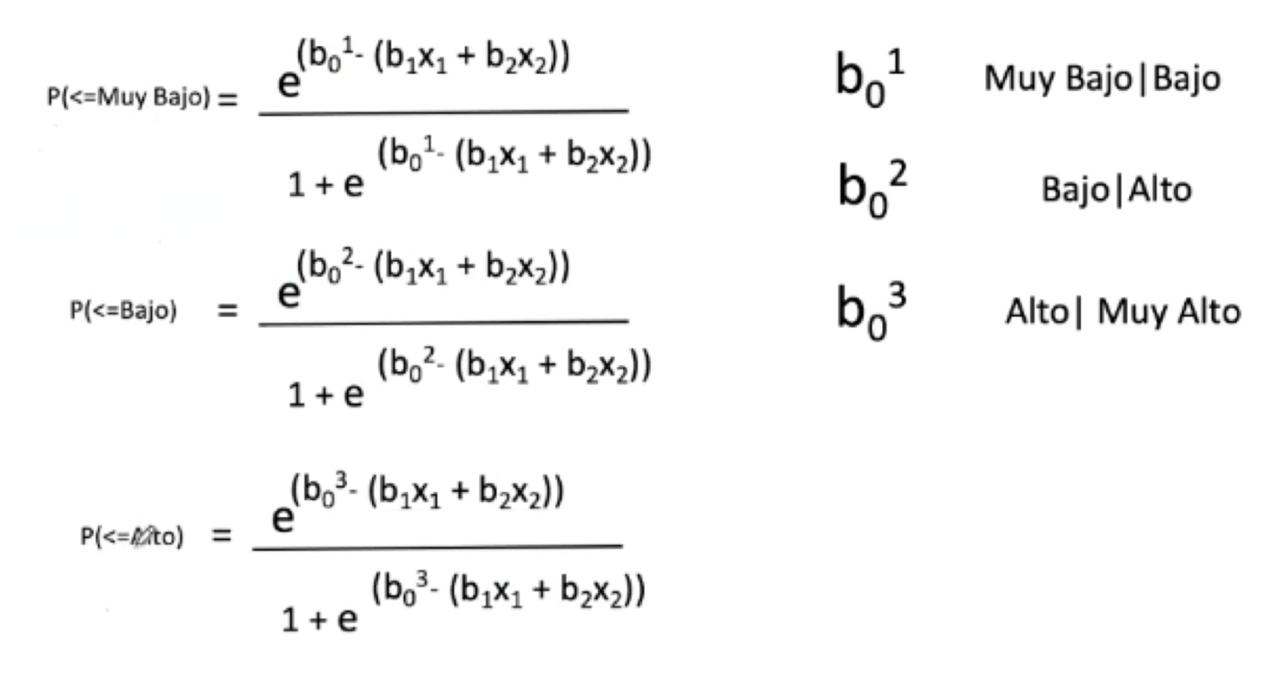
\includegraphics[width=0.8\linewidth]{EcuacionOrdinal} \end{center}

Recordamos los coeficientes

\begin{Shaded}
\begin{Highlighting}[]
\FunctionTok{coef}\NormalTok{(}\FunctionTok{summary}\NormalTok{(modelo))}
\end{Highlighting}
\end{Shaded}

\begin{verbatim}
##                    Value Std. Error   t value
## sexo_Mujer    -1.8362608 0.20267681 -9.060044
## educ           0.4618446 0.04136102 11.166180
## Muy Bajo|Bajo  3.6632440 0.55662857  6.581128
## Bajo|Alto      5.3305723 0.57522584  9.266921
## Alto|Muy Alto  7.1165070 0.62144567 11.451535
\end{verbatim}

\begin{center}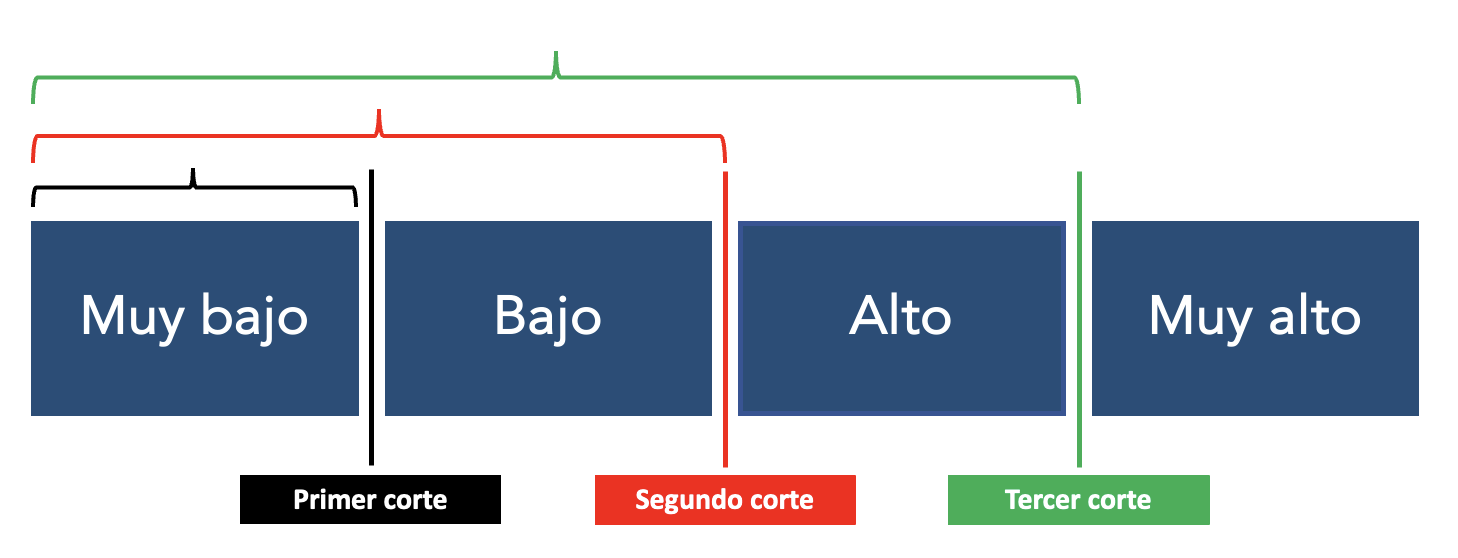
\includegraphics[width=0.8\linewidth]{Pd5_Cortes} \end{center}

\hypertarget{primer-corte-muy-bajo-bajo}{%
\paragraph{\texorpdfstring{\textbf{PRIMER CORTE: Muy Bajo \textbar{}
Bajo}}{PRIMER CORTE: Muy Bajo \textbar{} Bajo}}\label{primer-corte-muy-bajo-bajo}}

Hallemos primero la probabilidad del primer corte, que era Muy Bajo -
Bajo. Es decir, que la persona sea hombre con 15 años de educación tenga
un salario que sea menor o igual a muy bajo.

Reemplazamos los números de los coeficientes del corte de las variables
independientes.

\begin{Shaded}
\begin{Highlighting}[]
\NormalTok{num\_1 }\OtherTok{\textless{}{-}} \FunctionTok{exp}\NormalTok{(}\FloatTok{3.6632} \SpecialCharTok{{-}}\NormalTok{ ((}\SpecialCharTok{{-}}\FloatTok{1.8363}\SpecialCharTok{*}\DecValTok{0}\NormalTok{) }\SpecialCharTok{+}\NormalTok{ (}\FloatTok{0.4618}\SpecialCharTok{*}\DecValTok{15}\NormalTok{)))}
\NormalTok{denom\_1 }\OtherTok{\textless{}{-}} \DecValTok{1} \SpecialCharTok{+}\NormalTok{ num\_1}
\NormalTok{p\_menorigual\_muybajo}\OtherTok{\textless{}{-}}\NormalTok{ num\_1}\SpecialCharTok{/}\NormalTok{denom\_1}
\NormalTok{p\_menorigual\_muybajo}
\end{Highlighting}
\end{Shaded}

\begin{verbatim}
## [1] 0.03683416
\end{verbatim}

La probabilidad de que una persona que sea hombre y con 15 años de
educación tenga un salario menor o igual a Muy Bajo (solo muy bajo) es
de 0.036 o de 3.6\%

\begin{center}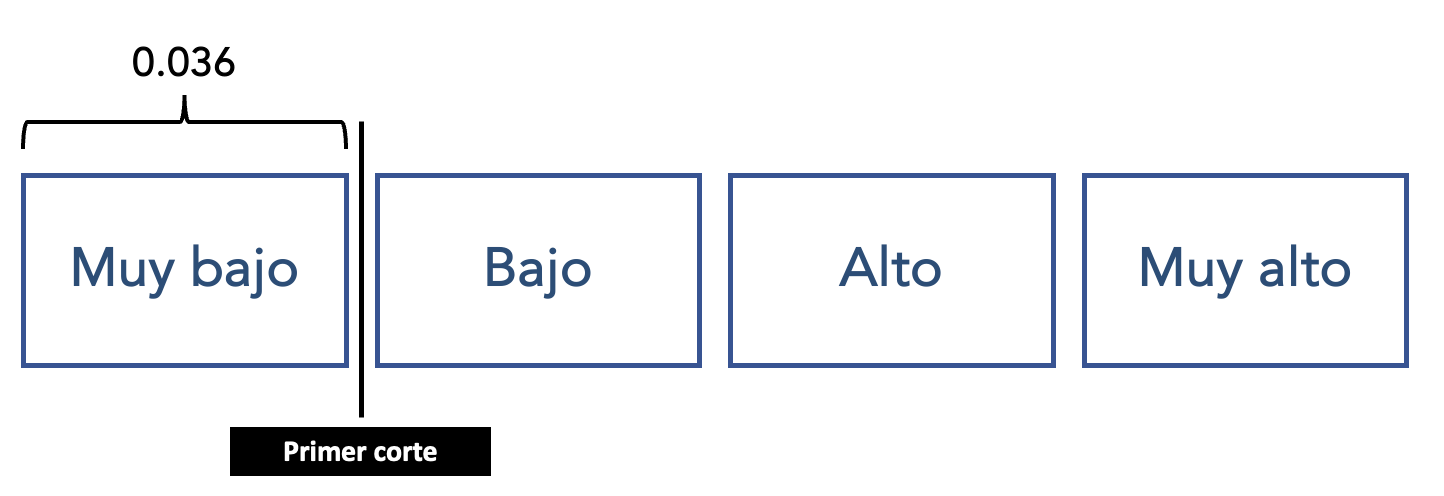
\includegraphics[width=0.8\linewidth]{pd5_corte1} \end{center}

\hypertarget{segundo-corte-bajo-alto}{%
\paragraph{\texorpdfstring{\textbf{SEGUNDO CORTE: Bajo \textbar{}
Alto}}{SEGUNDO CORTE: Bajo \textbar{} Alto}}\label{segundo-corte-bajo-alto}}

Ahora calculemos para todo lo que está por debajo de alto (menor o igual
a bajo); es decir, muy bajo y bajo.

\begin{Shaded}
\begin{Highlighting}[]
\NormalTok{num\_2 }\OtherTok{\textless{}{-}} \FunctionTok{exp}\NormalTok{(}\FloatTok{5.3306} \SpecialCharTok{{-}}\NormalTok{ ((}\SpecialCharTok{{-}}\FloatTok{1.8363}\SpecialCharTok{*}\DecValTok{0}\NormalTok{) }\SpecialCharTok{+}\NormalTok{ (}\FloatTok{0.4618}\SpecialCharTok{*}\DecValTok{15}\NormalTok{)))}
\NormalTok{denom\_2 }\OtherTok{\textless{}{-}}\NormalTok{ (}\DecValTok{1} \SpecialCharTok{+}\NormalTok{ num\_2)}
\NormalTok{p\_menorigual\_bajo}\OtherTok{\textless{}{-}}\NormalTok{num\_2}\SpecialCharTok{/}\NormalTok{denom\_2}
\NormalTok{p\_menorigual\_bajo}
\end{Highlighting}
\end{Shaded}

\begin{verbatim}
## [1] 0.1684854
\end{verbatim}

La probabilidad de que una persona que sea hombre y con 15 años de
educación tenga un salario menor o igual a bajo es de 0.16 o 16\%

\hypertarget{solo-probabilidad-de-bajo}{%
\paragraph{SOLO PROBABILIDAD DE BAJO}\label{solo-probabilidad-de-bajo}}

Se tiene la probabilidad de ser bajo y muy bajo, y previamente se hizo
la de muy muy bajo, estos se restan vas a tener la probabilidad de ser
únicamente bajo

\begin{Shaded}
\begin{Highlighting}[]
\NormalTok{p\_menorigual\_bajo}\SpecialCharTok{{-}}\NormalTok{p\_menorigual\_muybajo}
\end{Highlighting}
\end{Shaded}

\begin{verbatim}
## [1] 0.1316512
\end{verbatim}

La probabilidad de que una persona que sea hombre y con 15 años de
educación tenga un salario Bajo es de 0.13 o de 13.1\%

\begin{center}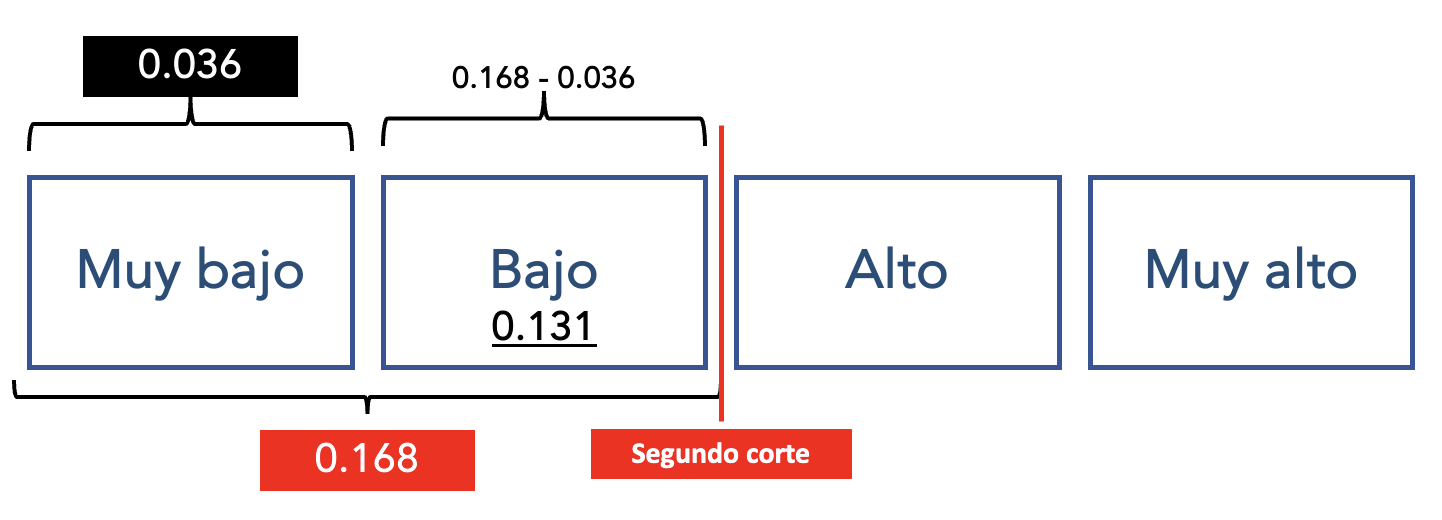
\includegraphics[width=0.8\linewidth]{pd5_corte2} \end{center}

\hypertarget{tercer-corte-alto---muy-alto}{%
\paragraph{\texorpdfstring{\textbf{TERCER CORTE: Alto - Muy
alto}}{TERCER CORTE: Alto - Muy alto}}\label{tercer-corte-alto---muy-alto}}

En este corte se calculan los tres escalones menores o iguales a alto:
Muy bajo, bajo y alto.

\begin{Shaded}
\begin{Highlighting}[]
\NormalTok{num\_3 }\OtherTok{\textless{}{-}}\FunctionTok{exp}\NormalTok{(}\FloatTok{7.1165} \SpecialCharTok{{-}}\NormalTok{ ((}\SpecialCharTok{{-}}\FloatTok{1.8363}\SpecialCharTok{*}\DecValTok{0}\NormalTok{) }\SpecialCharTok{+}\NormalTok{ (}\FloatTok{0.4618}\SpecialCharTok{*}\DecValTok{15}\NormalTok{)))}
\NormalTok{denom\_3 }\OtherTok{\textless{}{-}}\NormalTok{ (}\DecValTok{1} \SpecialCharTok{+}\NormalTok{ num\_3)}
\NormalTok{p\_menorigual\_alto}\OtherTok{\textless{}{-}}\NormalTok{num\_3}\SpecialCharTok{/}\NormalTok{denom\_3}
\NormalTok{p\_menorigual\_alto}
\end{Highlighting}
\end{Shaded}

\begin{verbatim}
## [1] 0.5472337
\end{verbatim}

La probabilidad de que una persona que sea hombre y con 15 años de
educación tenga un salario menor o igual a Alto - Bajo es de 0.54 o de
54\%.

\hypertarget{solo-probabilidad-de-alto}{%
\paragraph{SOLO PROBABILIDAD DE ALTO}\label{solo-probabilidad-de-alto}}

A la probabilidad de tener un nivel salarial menor o igual a alto
(resultado de tercer corte), le restamos la probabilidad de tener un
salario de nivel bajo, muy bajo (resultado de segundo corte).

\begin{Shaded}
\begin{Highlighting}[]
\NormalTok{p\_menorigual\_alto }\SpecialCharTok{{-}}\NormalTok{ p\_menorigual\_bajo}
\end{Highlighting}
\end{Shaded}

\begin{verbatim}
## [1] 0.3787484
\end{verbatim}

La probabilidad de que una persona que sea hombre y con 15 años de
educación tenga un salario Alto es de 0.378 o de 37.8\%

\begin{center}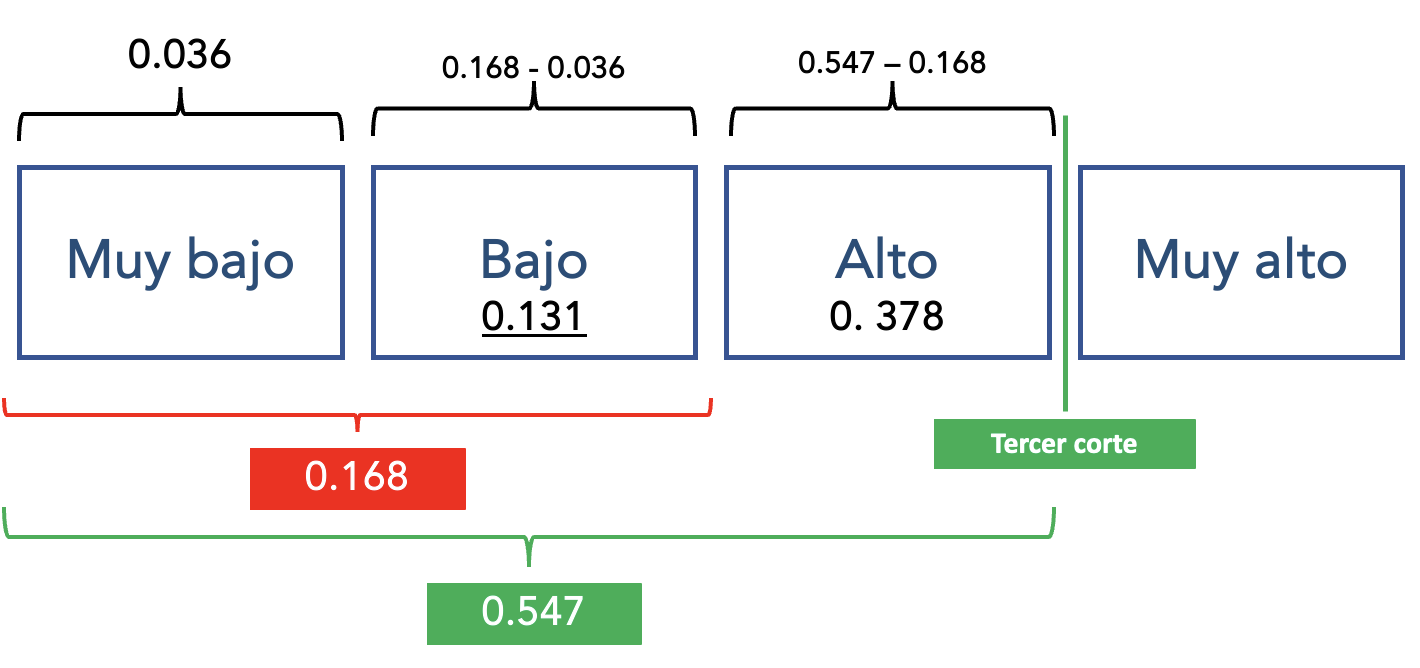
\includegraphics[width=0.8\linewidth]{pd5_corte3} \end{center}

\hypertarget{solo-probabilidad-de-muy-alto}{%
\paragraph{SOLO PROBABILIDAD DE MUY
ALTO}\label{solo-probabilidad-de-muy-alto}}

Como recordamos que era una probabilidad acumulada, donde llegaba hasta
MUY ALTO era 1. Ya tenemos la probabilidad de tener salario alto o
menos, para hallar la probabilidad de que sea muy alto, solo debemos
restar el resultado del tercer corte a 1 (1- Tercer corte)

\begin{Shaded}
\begin{Highlighting}[]
\DecValTok{1}\SpecialCharTok{{-}}\NormalTok{p\_menorigual\_alto}
\end{Highlighting}
\end{Shaded}

\begin{verbatim}
## [1] 0.4527663
\end{verbatim}

Entonces, la probabilidad de que una persona que sea hombre y con 15
años de educación tenga un salario Muy Alto es de 45.2\%

\begin{center}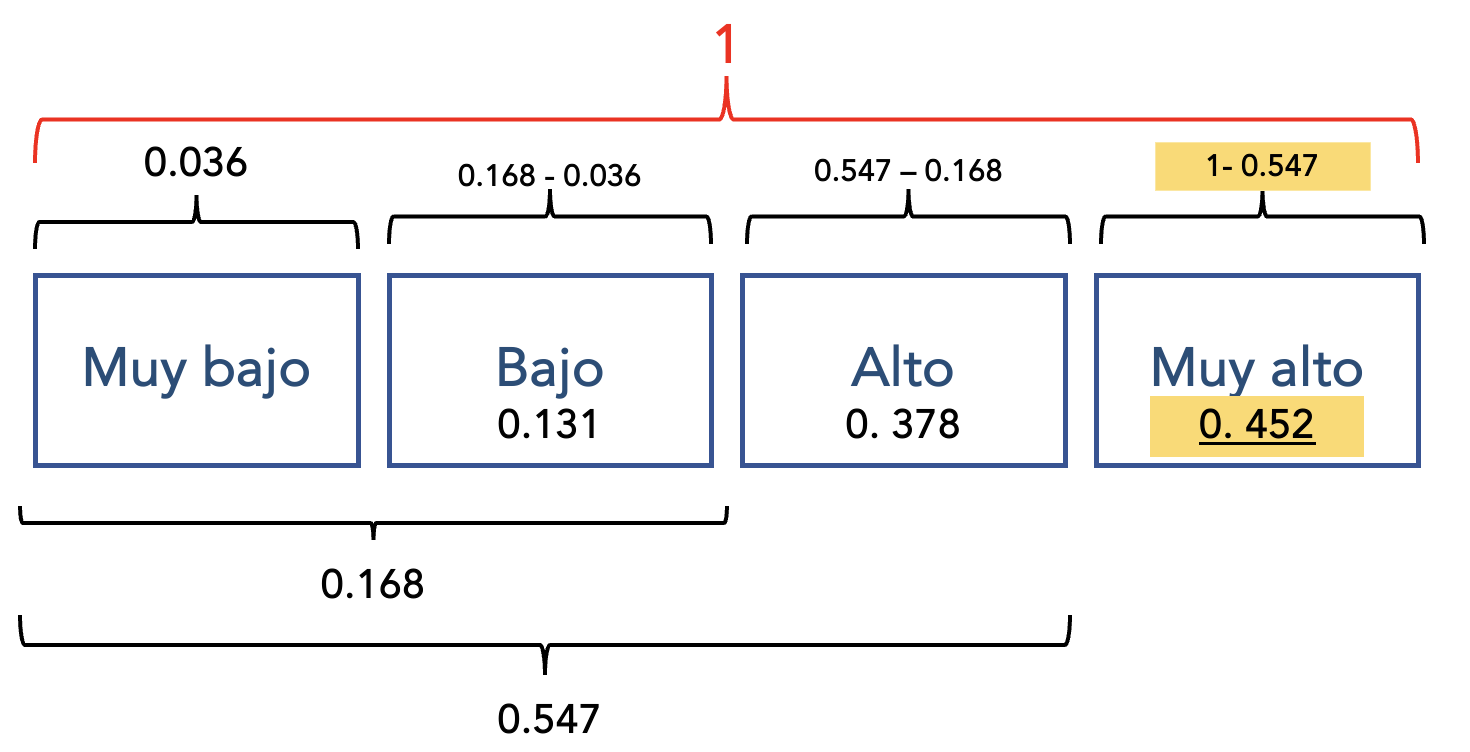
\includegraphics[width=0.8\linewidth]{pd5_muyalto} \end{center}

\hypertarget{modelo-2-de-quuxe9-manera-el-pertenecer-a-una-minoruxeda-ser-personal-administrativo-o-no-y-los-auxf1os-de-educaciuxf3n-condicionan-el-nivel-de-salario-que-puede-tener-un-trabajador}{%
\section{\texorpdfstring{\textbf{Modelo 2: ¿De qué manera, el pertenecer
a una minoría, ser personal administrativo o no y los años de educación
condicionan el nivel de salario que puede tener un
trabajador?}}{Modelo 2: ¿De qué manera, el pertenecer a una minoría, ser personal administrativo o no y los años de educación condicionan el nivel de salario que puede tener un trabajador?}}\label{modelo-2-de-quuxe9-manera-el-pertenecer-a-una-minoruxeda-ser-personal-administrativo-o-no-y-los-auxf1os-de-educaciuxf3n-condicionan-el-nivel-de-salario-que-puede-tener-un-trabajador}}

Convertir dummy a categoría laboral, ya que es politómica:

\begin{itemize}
\item
  0 es Ausente
\item
  1 es administrtivo
\item
  2 es seguridad
\item
  3 es directivo
\end{itemize}

\begin{Shaded}
\begin{Highlighting}[]
\FunctionTok{str}\NormalTok{(data}\SpecialCharTok{$}\NormalTok{catlab)}
\end{Highlighting}
\end{Shaded}

\begin{verbatim}
##  num [1:474] 3 1 1 1 1 1 1 1 1 1 ...
##  - attr(*, "label")= chr "Categoría laboral"
##  - attr(*, "format.spss")= chr "F1.0"
##  - attr(*, "labels")= Named num [1:4] 0 1 2 3
##   ..- attr(*, "names")= chr [1:4] "0 (Ausente)" "Administrativo" "Seguridad" "Directivo"
\end{verbatim}

\begin{Shaded}
\begin{Highlighting}[]
\FunctionTok{table}\NormalTok{(data}\SpecialCharTok{$}\NormalTok{catlab)}
\end{Highlighting}
\end{Shaded}

\begin{verbatim}
## 
##   1   2   3 
## 363  27  84
\end{verbatim}

\begin{Shaded}
\begin{Highlighting}[]
\NormalTok{data}\OtherTok{\textless{}{-}}\FunctionTok{dummy\_cols}\NormalTok{(data, }\AttributeTok{select\_columns =} \FunctionTok{c}\NormalTok{(}\StringTok{"catlab"}\NormalTok{))}
\end{Highlighting}
\end{Shaded}

Creación del modelo

\begin{Shaded}
\begin{Highlighting}[]
\NormalTok{modelo2 }\OtherTok{\textless{}{-}} \FunctionTok{polr}\NormalTok{(salario\_actual\_ordinal }\SpecialCharTok{\textasciitilde{}}\NormalTok{ minoría }\SpecialCharTok{+}\NormalTok{ catlab\_1 }\SpecialCharTok{+}\NormalTok{ educ, }\AttributeTok{data =}\NormalTok{ data, }\AttributeTok{Hess =}\NormalTok{ T)}
\FunctionTok{summary}\NormalTok{(modelo2)}
\end{Highlighting}
\end{Shaded}

\begin{verbatim}
## Call:
## polr(formula = salario_actual_ordinal ~ minoría + catlab_1 + 
##     educ, data = data, Hess = T)
## 
## Coefficients:
##            Value Std. Error t value
## minoría  -0.5621    0.21642  -2.597
## catlab_1 -3.6909    0.33029 -11.175
## educ      0.5170    0.04552  11.358
## 
## Intercepts:
##               Value    Std. Error t value 
## Muy Bajo|Bajo   1.9026   0.5828     3.2646
## Bajo|Alto       3.5595   0.6008     5.9242
## Alto|Muy Alto   5.7761   0.6355     9.0892
## 
## Residual Deviance: 909.0721 
## AIC: 921.0721
\end{verbatim}

Aplicar los pasos siguientes

\hypertarget{paso-5-quuxe9-modelo-es-el-muxe1s-ajustado}{%
\subsection{\texorpdfstring{\textbf{Paso 5: ¿Qué modelo es el más
ajustado?}}{Paso 5: ¿Qué modelo es el más ajustado?}}\label{paso-5-quuxe9-modelo-es-el-muxe1s-ajustado}}

\begin{Shaded}
\begin{Highlighting}[]
\FunctionTok{PseudoR2}\NormalTok{(modelo, }\AttributeTok{which =} \FunctionTok{c}\NormalTok{(}\StringTok{"Nagelkerke"}\NormalTok{))}
\end{Highlighting}
\end{Shaded}

\begin{verbatim}
## Nagelkerke 
##  0.5160308
\end{verbatim}

\begin{Shaded}
\begin{Highlighting}[]
\FunctionTok{PseudoR2}\NormalTok{(modelo2, }\AttributeTok{which =} \FunctionTok{c}\NormalTok{(}\StringTok{"Nagelkerke"}\NormalTok{))}
\end{Highlighting}
\end{Shaded}

\begin{verbatim}
## Nagelkerke 
##  0.6128653
\end{verbatim}

\end{document}
